\section{Kellerautomaten}

\begin{frame}{Kellerautomaten (PDA, i.Allg. nichtdeterministisch)}
	\begin{itemize}
		\item Grundidee Kellerautomat (PDA, push-down automaton)
		\begin{itemize}
			\item FA wird erweitert um einen zusätzlichen Kellerspeicher (Stack, Stapel)
			mit unbeschränkter Kapazität
			\item Stack: Datenstruktur mit den Methoden pop und push (LIFO-Prinzip)
			\item pop: oberstes Zeichen wird gelesen und gelöscht
			\item push: neues Zeichen wird auf den Stack geschrieben
		\end{itemize}
		\item Konfigurationsübergänge
		\begin{itemize}
			\item Nächstes Zeichen des Eingabewortes sowie oberstes Symbol auf Stack
			werden gelesen
			\item abhängig davon erfolgt Zustandsübergang, und es werden (i.Allg.
			mehrere) push-Operationen ausgeführt
			\item möglich sind auch $\varepsilon$-Übergänge: Zustandsübergang und Stack-
			Operationen ohne Weiterlesen des Eingabewortes
		\end{itemize}
	\end{itemize}
\end{frame}

\begin{frame}{Spezifikation PDA}
	\begin{itemize}
		\item Spezifikation nichtdeterministischer PDA\\
		$A_{PDA}=(S, \Sigma, \Gamma, \delta, s_0, \#, F)$
		\begin{itemize}
			\item $S$: Zustandsmenge
			\item $\Sigma$: Terminalalphabet
			\item $\Gamma$: Kelleralphabet
			\item $\delta$: Zustandsüberführungsrelation, $\delta \subseteq S \times \Sigma \times \Gamma \times S \times \Gamma^*$
			\item $\#$: Kellerboden-Symbol, $\# \in \Gamma$
			\item $s_0$: Startzustand, $s_0 \in S$
			\item $F$: Menge von Endzuständen
		\end{itemize}
		\item Konfiguration: $(s, u, \gamma)$
		\item Konfigurationsübergang: $(s_1, av, A\beta) \mapsto (s_2, v, \alpha\beta)$
	\end{itemize}
	\centering
	\begin{tikzpicture}
		\node[state] (s1) {$s_1$};
		\node[state, right=of s1] (s2) {$s_2$};
		
		\draw (s1) edge[above] node{$a, A/\alpha$} (s2);
	\end{tikzpicture}
\end{frame}

\begin{frame}{Akzeptierte Sprache}
	\begin{itemize}
		\item Akzeptanzverhalten
		\begin{itemize}
			\item per Endzustand akzeptierte Sprache\\
			$L(A)=\{w \in \Sigma^* \mid (s_0, w, \#) \mapsto^* (s_f, \varepsilon, \beta), s_f \in F, \beta \in \Gamma^*\}$\\
			d.h. Keller muss nicht leer sein
			\item durch leeren Keller akzeptierte Sprache\\
			(beachte: auch der Kellerboden wird gelöscht!)\\
			$L_\varepsilon(A)=\{w \in \Sigma^*\mid (s_0, w, \#) \mapsto^* (q, \varepsilon, \varepsilon), q \in S\}$\\
			d.h. Zustand am Wortende kann beliebig sein
		\end{itemize}
		\item die beiden Akzeptanzbedingungen sind wie folgt äquivalent:
		\begin{itemize}
			\item zu jedem nichtdet. PDA $K$ gibt es einen PDA $K'$ mit $L(K) = L_\varepsilon(K')$
			\item zu jedem nichtdet. PDA $K$ gibt es einen PDA $K'$ mit $L(K') = L_\varepsilon(K)$
		\end{itemize}
	\end{itemize}
\end{frame}

\begin{frame}{Zusammenhang mit kontextfreien Sprachen}
	\begin{itemize}
		\item zu jedem PDA lässt sich eine kontextfreie Grammatik konstruieren, die die gleiche Sprache generiert (siehe Folie \ref{Grammatik_aus_PDA})
		\item zu jeder kontextfreien Grammatik lässt sich ein (i.Allg. nichtdeteministischer) PDA konstruieren, der die gleiche Sprache akzeptiert
		\item Grundsätzlicher Zusammenhang mit kontextfreier Grammatik
		\begin{itemize}
			\item PDA kann mit Grammatik-Startsymbol $S$ als Kellerboden initialisiert werden
			\item liegt Variable A oben auf Stack: per $\varepsilon$-Übergang durch rechte Seite einer Regel ersetzen (Produktion anwenden, dabei nichtdeterministisch raten)
			\item liegt Terminalsymbol $a$ oben auf Stack: mit gelesenem Symbol abgleichen; Löschen bei Übereinstimmung, sonst Kopie verwerfen (matching Kellertop mit aktuellem Eingabezeichen)
			\item Äquivalenter PDA ist i.Allg. nichtdeterministisch; lässt sich i.Allg. \underline{nicht} in einen deterministischen PDA äquivalent umrechnen
		\end{itemize}
	\end{itemize}
\end{frame}

\note{
	Nachfolgendes Beispiel: $$P=\{ S\rightarrow \varepsilon \mid X, \quad X \rightarrow aXa\mid bXb \mid aa \mid bb\}$$
}

\begin{frame}{Beispiel: Umwandlung Typ-2-Grammatik $\rightarrow$ Kellerautomat}
	Grammatik:
	$$P=\{ S\rightarrow \varepsilon \mid X, \quad X \rightarrow aXa\mid bXb \mid aa \mid bb\}$$
	Kellerautomat:\\
	\centering
	\begin{tikzpicture}
		\node[state, initial] (s0) {$s_0$};
		\node[state, right=of s0] (s1) {$s_1$};
		\node[state, accepting, below=of s1] (s2) {$s_2$};
		
		\draw (s0) edge[above] node{$\varepsilon, \#/S\#$} (s1)
			  (s1) edge[loop right, align=center] node{
			  										$a,a/\varepsilon$\\
			  										$b,b/\varepsilon$\\
			  										$\varepsilon,X/bb$\\
		  											$\varepsilon,X/aa$\\
		  											$\varepsilon,X/bXb$\\
		  											$\varepsilon,X/aXa$\\
		  											$\varepsilon,S/X$\\
  													$\varepsilon,S/\varepsilon$} (s1)
  			  (s1) edge[left] node{$\varepsilon,\#/\#$} (s2);
	\end{tikzpicture}
\end{frame}

\note{
	Sprache: Palindrome gerader Länge $L=\{w\tilde{w} \mid w \in \{a,b\}^*\}$
}

\begin{frame}{PDA, der mit leerem Keller akzeptiert $\rightarrow$ kontextfreie Grammatik}
	\label{Grammatik_aus_PDA}
	\begin{columns}
		\column{.5\textwidth}
		Regeln
		\begin{itemize}
			\item Startregel\\
			$S\rightarrow [s_0, \#, s_i]$ für alle $s_i \in S$
			\item Übergang $(s_j,a,A,s_k,B_1\ldots B_m)$\\
			$[s_j,A,s_{m+1}] \rightarrow a[s_k,B_1,s_l]\ldots[s_m,B_m,s_{m+1}]$ für alle Kombinationen $s_l,\ldots,s_{m+1}$
			\item Übergang $(s_j,a,A,s_k,\varepsilon)$\\
			$[s_j,A,s_k]\rightarrow a$
		\end{itemize}
		\column{.5\textwidth}
		Beispiel $L=\{a^nb^n \mid n \geq 1\}$\\
		 $\delta=\{(s_0,a,\#,s_0,A),(s_0,a,A,s_0,AA),$\\
		 \qquad$(s_0,b,A,s_1,\varepsilon),(s_1,b,A,s_1,\varepsilon)\}$\\
		 \vspace{0.5em}
		Regeln: $P=\{S \rightarrow [s_0,\#,s_0]|[s_0,\#,s_1],$\\
			$[s_0,\#,s_0]\rightarrow a[s_0,A,s_0],$\\
			$[s_0,\#,s_1]\rightarrow a[s_0,A,s_1],$\\
			$[s_0,A,s_0]\rightarrow a[s_0,A,s_0][s_0,A,s_0],$\\
			$[s_0,A,s_0]\rightarrow a[s_0,A,s_1][s_1,A,s_0],$\\
			$[s_0,A,s_1]\rightarrow a[s_0,A,s_0][s_0,A,s_1],$\\
			$[s_0,A,s_1]\rightarrow a[s_0,A,s_1][s_1,A,s_1],$\\
			$[s_0,A,s_1]\rightarrow b,$\\ $[s_1,A,s_1]\rightarrow b\}$
	\end{columns}
\end{frame}

\begin{frame}{Berechnung: PDA, der mit leerem Keller akzeptiert $\rightarrow$ kontextfreie Grammatik}
	\begin{columns}
		\column{.4\textwidth}
		\begin{tikzpicture}
			\node[state, initial] (s0) {$s_0$};
			\node[state, right=of s0] (s1) {$s_1$};
			\draw	(s0) edge[loop above] node{$a, \#/A$} (s0)
			(s0) edge[loop below] node{$a, A/AA$} (s0)
			(s0) edge[above] node{$b, A/\varepsilon$} (s1)
			(s1) edge[loop above] node{$b,A/\varepsilon$} (s1);
		\end{tikzpicture}
		\begin{tabular}{ccccccccccccc}
			& a &  & a &  & b &  & b &  \\
			\hline
			&  &  &  & A &  &  &  &  \\
			\# &  & A &  & A &  & A &  &  \\
			\hline
			$s_0$ &  & $s_0$ &  & $s_0$ &  & $s_1$ &  & $s_1$ \\
		\end{tabular}
		\column{.6\textwidth}
		\begin{itemize}
			\item Kodierung von "`Aufgaben"'
			\item Hauptaufgabe: Keller soll leer werden\\
			Starten in $s_0$, \# soll "`abgebaut"' werden, Folgezustand ist egal: $[s_0, \#, s_0]$ bzw. $[s_0, \#, s_1]$
			\item Kodierungen werden als Nichtterminalsymbole (aka Variablen) interpretiert\\
			Startregeln: $S \rightarrow [s_0, \#, s_0]|[s_0, \#, s_1]$
			\item analog Kodierung aller weiteren Übergänge des Automaten als Regeln, z.B. führt das Lesen eines $b$ im Zustand $s_0$ zum Abbau eines $A$ auf dem Stack und Übergang in $s_1$:\\
			$[s_0, A, s_1] \rightarrow b$
		\end{itemize}
	\end{columns}
\end{frame}

\begin{frame}{Deterministische Kellerautomaten (DPDA): Problemstellung}
	\begin{itemize}
		\item Für praktische Anwendungen (Parser) wird ein im wesentlichen lineares Laufzeitverhalten angestrebt
		\item Die Simulation nichtdeterministischer Automaten zeigt i.Allg. ein exponentielles Verhalten
		\item Lässt sich jeder nichtdet. Kellerautomat in einen äquivalenten det. Kellerautomaten umschreiben?\\
		\underline{nein:} z.B. $L=\{w\tilde{w} \mid w\in \Sigma^*\}$ ist kontextfrei, aber nicht durch det. PDA akzeptierbar
		\item \underline{Deterministisch kontextfreie Sprachen} sind solche, die durch einen deterministischen Kellerautomaten (per Endzustand) akzeptiert werden. Sie bilden damit eine \underline{Unterklasse} der kontextfreien Sprachen.
	\end{itemize}
\end{frame}

\begin{frame}{Deterministische Kellerautomaten}
	\begin{itemize}
		\item Spezifikation:\\
		deterministische Zustandsüberführungsfunktion; \underline{$\varepsilon$-Übergänge erlaubt}\\
		insoweit gilt (für $a \in \Sigma, A \in \Gamma$): $|\delta(s, a, A)| + |\delta(s, \varepsilon, A)| \leq 1$ (d.h.: für	jede Konfiguration $(s, ax, A\rho)$ gibt es höchstens eine Folgekonfiguration)
		\item Nichtäquivalenz von Akzeptanz per leerem Keller bzw.
		Endzustand bei det. PDA:\\
		führt bei DPDA \underline{nicht} zur gleichen Sprachklasse
		\item Definition: Präfixeigenschaft\\
		Die Sprache $L$ hat die Präfixeigenschaft gdw. für alle $w \in L$ gilt:\\
		Ist $x$ echtes Präfix von $w$ (d.h. $w=xy, y \neq \varepsilon$) dann gilt $x \notin L$
		\item Es gilt: deterministisch kontextfreie Sprachen, die durch	DPDA per leerem Keller akzeptiert werden können, sind genau die mit Präfixeigenschaft
	\end{itemize}
\end{frame}

\begin{frame}{Beziehungen zwischen Sprachklassen}
	\begin{itemize}
		\item Die det. kontextfreien Sprachen $L_\varepsilon(A)$ (mit Präfixeigenschaft, Akzeptanz per leerem Keller) sind echt in den det. kontextfreien Sprachen $L(A)$ (Akzeptanz per Endzustand) enthalten
		\item \underline{reguläre} Sprachen sind echt in den det. kontextfreien	Sprachen enthalten ( FA ist "`Kellerautomat ohne Keller"')
		\item es gibt \underline{reguläre} Sprachen, die die Präfixeigenschaft nicht besitzen und damit in $L_\varepsilon(A)$ nicht enthalten sind (z.B. $\alpha=a|ab$)
		\item es gibt \underline{reguläre} Sprachen, die die Präfixeigenschaft besitzen und damit in $L_\varepsilon(A)$ liegen (z.B. $\alpha=a|ba$)
		\item es gibt Sprachen in $L_\varepsilon(A)$, die nicht regulär sind (z.B ${a^nb^n}$)
	\end{itemize}
\end{frame}

\begin{frame}{Exkurs: (N)FA im RL}
Pac-Man \footnote{Applications of Deterministic Finite Automata, Eric Gribkoff, \url{https://www.cs.ucdavis.edu/~rogaway/classes/120/spring13/eric-dfa.pdf}}
		\begin{columns}
			\column{.5\textwidth}
		\begin{figure}
			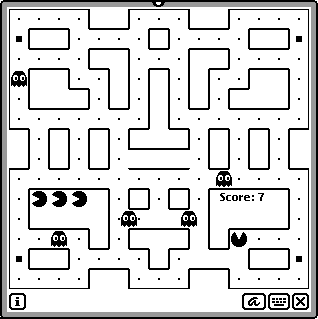
\includegraphics[width=0.6\linewidth]{images/Pac-Man}
		\end{figure}
		\column{.8\textwidth}
		\begin{tikzpicture}
			\node[state, initial] (w) {wander};
			\node[state, right=3cm of w] (c) {chase};
			\node[state, below=of w] (r) {return};
			\node[state, below=of c, right=3.24cm of r]  (f) {flee};
			
			\draw
				(w) edge[bend left=10, above] node{PM spotted} (c)
				(w) edge[bend left=10, above] node{PM power-up} (f)
				(c) edge[bend left=10, below] node{lost PM} (w)
				(c) edge[right] node{PM power-up} (f)
				(f) edge[bend left=10, below] node{PM power-dn} (w)
				(f) edge[below] node{eaten by PM} (r)
				(r) edge[left] node{reach base} (w);
		\end{tikzpicture}
	\end{columns}
\end{frame}

\begin{frame}{Exkurs: PDA im RL}
	Drehkreuz
	\begin{center}
		\begin{figure}
			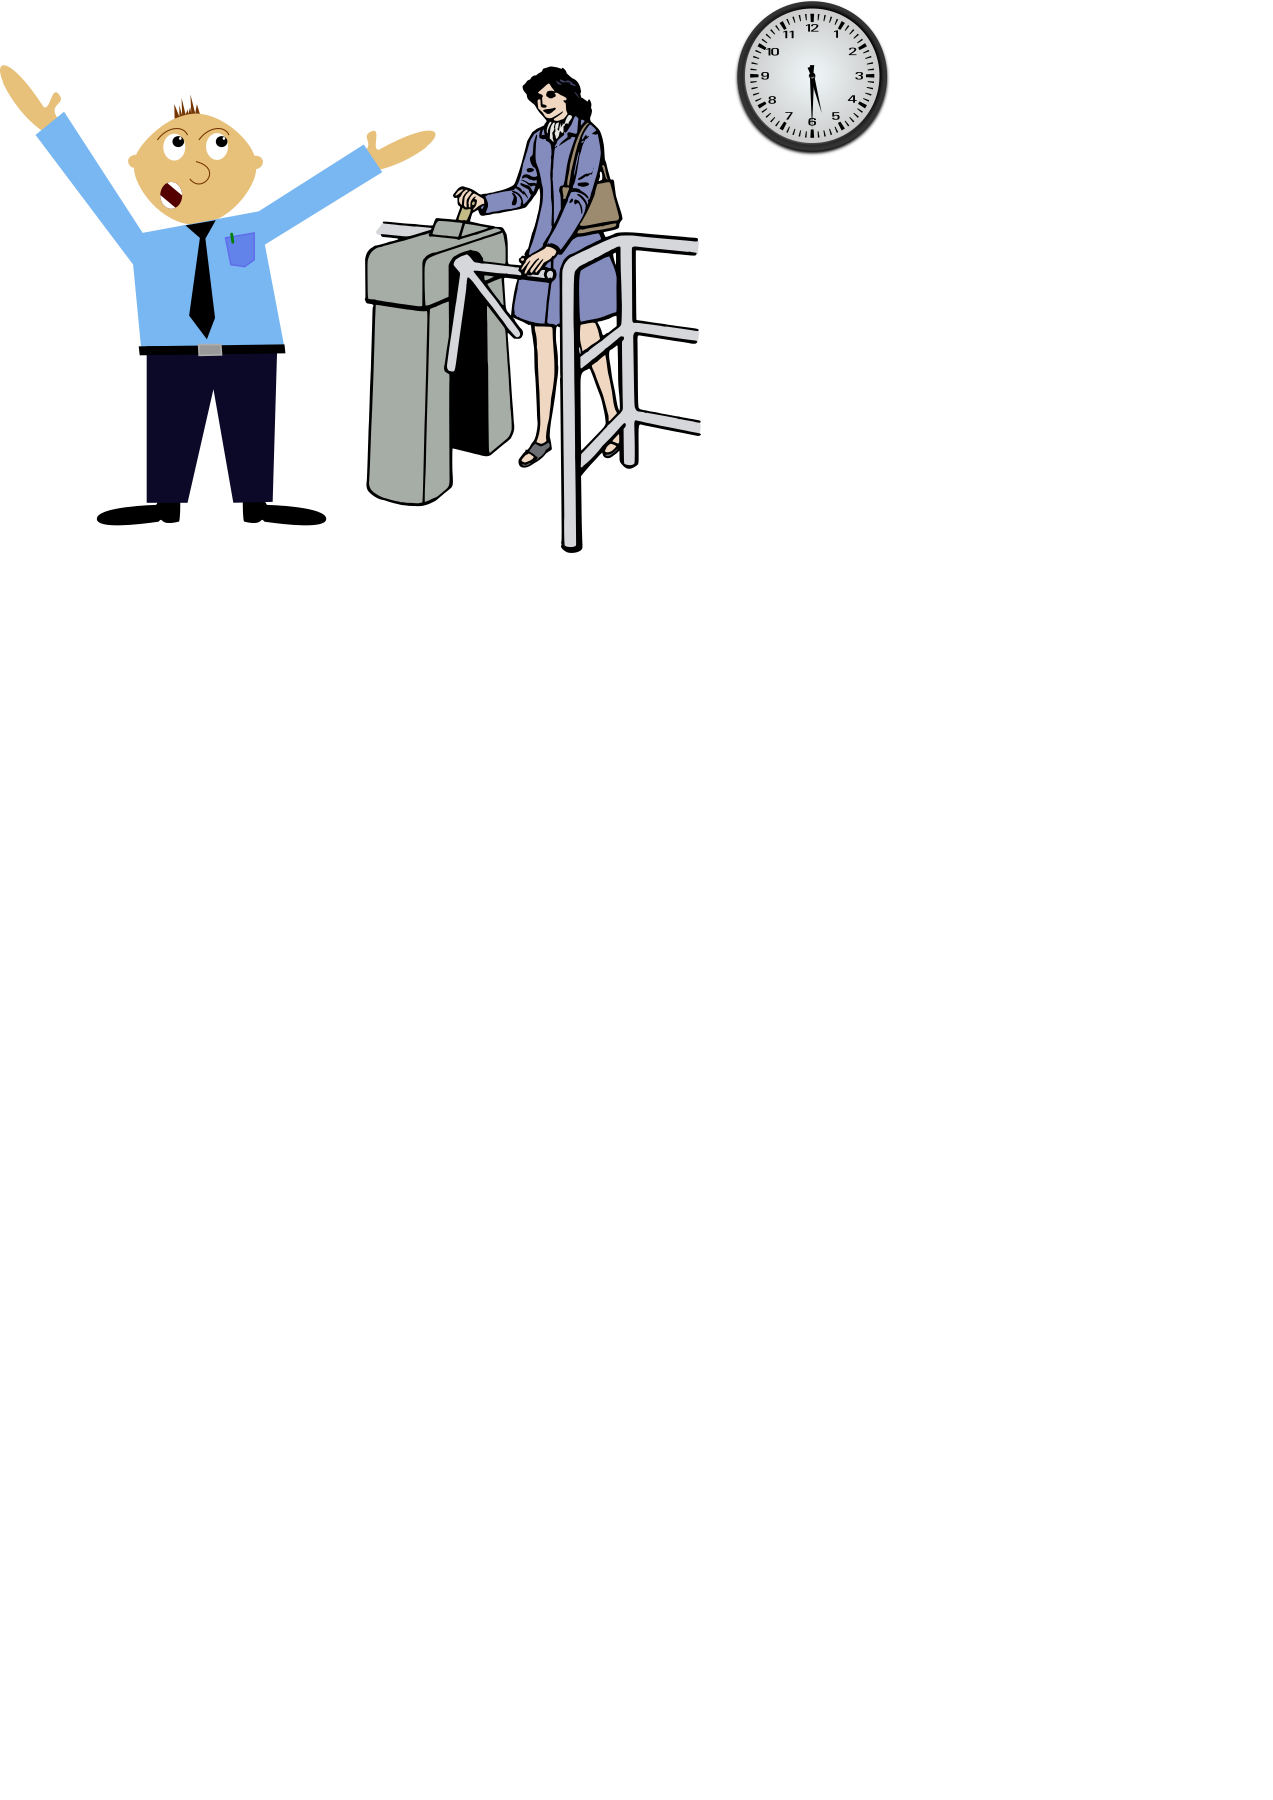
\includegraphics[width=\linewidth]{images/turnstile}
		\end{figure}
	\end{center}
\end{frame}